\documentclass[12pt,a4paper]{article}
\usepackage[utf8x]{inputenc}
\usepackage{amsmath}
\usepackage{amsfonts}
\usepackage{graphicx}
\usepackage{float}
\usepackage{amsthm}
\usepackage{lipsum}
\usepackage{bbm}
\newtheoremstyle{break}
{\topsep}{\topsep}%
{\itshape}{}%
{\bfseries}{}%
{\newline}{}%
\theoremstyle{break}
\newtheorem{remark}{Remark}
%opening
\title{Extensions}
\author{}

\begin{document}

\maketitle

\begin{abstract}
	Si presentano due estensioni alla teoria in ambito Event-Driven. Partendo sempre dal modello del Dott.Specchio, prima si suppone una dinamica GBM per il risky asset, poi invece si suppone una dinamica di tasso per il risk-free asset (cash). Infine si mostra come questi due approcci possono essere uniti per avere sia dinamica di tasso che dinamica GMB per risky asset
\end{abstract}

\section{Dinamica GBM per risky asset}
Si suppone un portfolio composto da cash (100\%) più risky asset (esposizione a future su indice). Si suppone inoltre la seguente dinamica per il risky asset 
\[
\begin{cases}
dS_t = \mu S_tdt + \sigma S_t dW_t  \\
S(t_0) = S_{t_0}
\end{cases}
\]
in cui $\{W_t\}_{t\geq0}$ è un moto Browniano unidimensionale. Risolvendo L'SDE si ha 
\begin{align}
S_t & = S_{t_0} \exp\big((\mu - \frac{\sigma^2}{2})(t - t_0) + \sigma (W_t - W_{t_0})\big) \\
    & = S_{t_0} \exp\big(\tilde{\mu}(t - t_0) + \sigma (W_t - W_{t_0})\big)
\end{align}

Definisco $\{X_t\}_{t\geq t_0}$ il rendimento del risky asset a partire dall'istante $t_0$ nella seguente maniera \[ X_t = \log(S_t/S_{t_0}) = \tilde{\mu}(t - t_0) + \sigma (W_t - W_{t_0})
\]
Siccome  si vuole modellizzare non tanto l'istante in cui avviene l'evento, ma bensì la durata tra due eventi consecutivi (durata dell' holding time) si ridefinisce il processo rendimento del modo seguente\footnote{equivale a shiftare il processo indietro all'istante 0. Intuitivamente questo è lecito in quanto il moto Browniano ha incrementi stazionari} \[ X_t := \log(S_{t + t_0}/S_{t_0}) = \tilde{\mu}t + \sigma \big(W_{t + t_0} - W_{t_0}\big) = \tilde{\mu}t + \sigma\widetilde{W}_{t} \quad t \geq 0
\]
dove si è usato la proprietà che $\widetilde{W}_t = W_{t + t_0} - W_{t_0}$ è ancora un moto Browniano rispetto alla filtrazione $\mathcal{F}_{t + t_0}$. Osservo quindi che il rendimento del risky asset è un moto Browniano con drift (processo per cui ho teoria dei tempi d'uscita)
\subsection{densità $\tau_{k+1}$}
Si supponga $t_k$ sia l'istante in cui il k-esimo evento accade. Si ricorda che si ha un evento non appena il modulo del rendimento del risky asset ($X_t)$  supera quota $J$. Si è interessati a modelizzare  $\tau_{k+1}$, ossia l'holding time tra il k-esimo e il k+1-esimo evento. In particolare, si definisce il seguente tempo d'arresto
\begin{align*}
\tau_{k+1} & := \inf\{t\geq 0 : \quad |X_t| \geq J \} = && \text{(definizione)}\\
& = \inf\{t\geq 0 : \quad X_t \notin (-J,J) \} = \\
& = \inf\{t\geq 0 : \quad |\log(\frac{S_{t_k + t}}{S_{t_k}})| \geq J \} =\\
& = \inf\{t\geq 0 : \quad |\tilde{\mu} t + \sigma \widetilde{W}_t| \geq J \}
\end{align*}


Si è interessati a conoscere la distribuzione della v.a. $\tau_{k+1}$. In calcolo stocastico questo è un problema noto che va sotto il nome di  \textit{double exit problem} per un moto Browniano con drift. (\cite{PassTime}) fornisce il seguente fondamentale risultato :

\begin{align*}
F_{\tau_{k+1}}(t) & = \mathbb{P}\Big(\tau_{k+1}\leq t \Big) = 1 - \big[ \exp(-\tilde{\mu}J / \sigma^2) K_t^\infty(J) - \exp(\tilde{\mu}J / \sigma^2) K_t^\infty(-J)\big] \\
& = 1-\big[2\cosh(\tilde{\mu}J / \sigma^2)K_t^\infty(J)\big]
\end{align*}

con
\[
K_t^N(k) = \frac{\sigma^2\pi}{4J^2}\sum_{n=1}^{N}\frac{n(-1)^{n+1}}{\big(\frac{\tilde{\mu}}{2\sigma^2} + \frac{\sigma^2n^2\pi^2}{8J^2}\big)}\exp\Big(-\big(\frac{\tilde{\mu}}{2\sigma^2} + \frac{\sigma^2n^2\pi^2}{8J^2}\big)t\Big) \sin\big(\frac{n\pi k}{2J}\big)
\]

\subsection{densità $X_{\tau_{k+1}}$}
La dinamica di portfolio in ottica event-driven si scrive quindi
\begin{equation}\label{ptfDyn}
\boxed{x_{k+1} = x_k \big(\exp\{r \tau_{k+1}\} + u_k X_{\tau_{k+1}}\big)}
\end{equation}
dove la v.a. $X_{\tau_{k+1}}$ non è altro che il processo rendimento arrestato all'istante aleatorio $\tau_{k+1}$, $r$ è il rendimento costante del cash e $u_k$ il del peso del risky asset.
$X_{\tau_{k+1}}$ può assumere solo due valori (-$J$ o $J$) quindi $X_{\tau_{k+1}} \sim \text{B}(p)$. Si dimostra\footnote{esercizio in \cite{Baldi}} che
\begin{equation}
\mathbb{P}\Big(X_{\tau_{k+1}} = J\Big) := p = \frac{1-e^{2\tilde{\mu}J/\sigma^2}}{e^{-2\tilde{\mu}J/\sigma^2} - e^{2\tilde{\mu}J/\sigma^2}} = \frac{e^{2\tilde{\mu}J/\sigma^2}-1}{2\sinh(2\tilde{\mu}J/\sigma^2)}
\end{equation}

\subsection{sintesi}
Infine si vuole calcolare la densità della v.a. in (\ref{ptfDyn}) che poi sarà la funzione da inserire nell'algoritmo ODAA. Svolgendo tutti i calcoli e sfruttando la disparità di $K_t^\infty(k)$ in $k$ si ottiene\footnote{a meno di errori e omissioni}
\begin{equation}
f_{x_{k+1}}(z) = \frac{2\cosh\big(\frac{\tilde{\mu}J}{\sigma^2}\big)}{rx}\Big[p \Gamma^\infty_{\frac{z-\xi}{x}}(J) \mathbbm{1}_{[x+\xi,\infty)} + (1-p)\Gamma^\infty_{\frac{z+\xi}{x}}(J) \mathbbm{1}_{[x-\xi,\infty)}  \Big]
\end{equation}
dove $\xi = x u_k J$ e 
\begin{align*}
\Gamma^\infty_{z}(J) &= -\frac{d}{dz}\Big(K^\infty_{\frac{1}{r}\log(z)}(J)\Big)\\
&=\frac{\sigma^2\pi}{4J^2}\sum_{n=1}^{\infty}n(-1)^{n+1}z^{\Big(-\big(\frac{\tilde{\mu}}{2\sigma^2} + \frac{\sigma^2n^2\pi^2}{8J^2}\big)-1\Big)}\sin(\frac{\pi}{2}n)
\end{align*}
\section{Dinamica tasso}
L'obiettivo di questa sezione è introdurre una dinamica di tasso per il cash. Si suppone che il cash evolva con la seguente dinamica 
\[
\begin{cases}
dB(t) = r(t)B(t)dt \\  
B(t_0) = 1
\end{cases}
\]
ossia \[ B(t) = \exp\Big(\int_{t_0}^{t}r(s)ds\Big) := \exp(v_t)\] Per lo short-rate $r_t$ si sceglie il modello di Vasicek

\begin{equation}\label{Vas1}
\begin{cases}
dr_t = a(b - r_t)dt + \sigma dW_t\\
r_{t_0} = r_0
\end{cases}
\end{equation}

Risolvendo questa SDE si ha
\begin{equation}\label{Vas2}
r_t = r_0e^{-a(t-t_0)} + b \big(1-e^{-a(t-t_0)}\big)+\sigma e^{-a (t-t_0)}\int_{t_0}^{t}e^{a(s-t_0)}dW_s
\end{equation}
Si vuole trovare una forma esplicita del processo Integrated Ornstein–Uhlenbeck $v_t$. Integrando la (\ref{Vas1}) su $[t_0,t]$ e uguagliando alla (\ref{Vas2}) si ottiene 
\begin{equation}
	\boxed{v_t = \frac{1}{a}\Big[(r_0 - b)\big(1-e^{-a(t-t_0)}\big)+ab(t-t_0)+\sigma\int_{t_0}^{t}\big(1-e^{-a(t-s)}\big)dW_s  \Big]}
\end{equation}
A questo punto, una volta fissato $t \in \mathbb{R}^+$, posso calcolare la legge della v.a. $v_t$ e ottenere
\[
v_t \sim \mathcal{N}
\]
\[
\mathbb{E}[v_t] = \frac{1}{a}\Big[(r_0 - b)\big(1-e^{-a(t-t_0)}\big)+ab(t-t_0)\Big]
\]
\[
Var[v_t] = \frac{\sigma^2}{2a^3}\Big[2a(t-t_0) + 4e^{-a(t-t_0)}-e^{-2a(t-t_0)}-3\Big]
\]

\begin{remark}
	I parametri della v.a. $v_t$  non dipendono dal particolare intervallo di tempo che considero ma solamente dalla lunghezza $t-t_0$, che è proprio quello si vuole modellizare con il tempo d'arresto $\tau_{k+1}$
\end{remark}
Posso quindi ridefinire $v_t := \int_{t_k}^{t_k+t}r(s)ds$ e avere
\[
\mathbb{E}[v_t] = \frac{1}{a}\Big[(r_0 - b)\big(1-e^{-at}\big)+abt\Big] := \tilde{\eta}(t)
\]
\[
\text{Var}[v_t] = \frac{\sigma^2}{2a^3}\Big[2at + 4e^{-at}-e^{-2at}-3\Big] := \tilde{\sigma}(t)
\]
ossia ho i parametri in funzione della realizzazione dell'holding time $\tau_{k+1} = t$

\subsection{densità $x_{k+1}$}

Sia $t_k$ l'istante in cui il k-esimo evento accade, la dinamica del valore di porfolio può essere espressa nella seguente maniera
\begin{align*}
x_{k+1} & = x_k \Big(\exp\big(\int\limits_{t_k}^{t_k+\tau_{k+1}}r(s)ds\big) + u_k J \Delta\widetilde{N}\Big) = \\
& = x_k \Big(\exp(v_{\tau_{k+1}}) + u_k J \Delta\widetilde{N}\Big)
\end{align*}

Svolgendo tutti i conti si ottiene infine la densità desiderata 
\begin{align}
f_{x_{k+1}}(z) &= p\Bigl\{ \int_{0}^{\infty}\phi\Big(\frac{\log\big(\frac{z-\xi}{x}\big)-\tilde{\eta}(t)}{\tilde{\sigma}(t)}\Big)  \Big(\frac{1}{\tilde{\sigma}(t)(z-\xi)}\Big)f_{\tau_{k+1}}(t)dt\Bigr\}\mathbbm{1}_{[x+\xi,\infty)} \nonumber +\\
& + (1-p)\Bigl\{ \int_{0}^{\infty}\phi\Big(\frac{\log\big(\frac{z+\xi}{x}\big)-\tilde{\eta}(t)}{\tilde{\sigma}(t)}\Big)  \Big(\frac{1}{\tilde{\sigma}(t)(z+\xi)}\Big)f_{\tau_{k+1}}(t)dt\Bigr\}\mathbbm{1}_{[x-\xi,\infty)}
\end{align}
avendo indicato con $\phi$ la pdf di una normale standard e $\xi= xJu$
\begin{remark}
	Questa formula è generale nel senso che $p$ e $f_{\tau_{k+1}}$ possono essere sia quelli del modello base ma anche quelli ricavati nella sezione precedente e quindi con l'ipotesi di una dinamica GBM per il risky asset.
\end{remark}

\begin{remark}
	Ulteriori questioni non riportate qui sono la calibrazioine dei modelli. Per calibrare il GMB si ricavano stimatori espliciti per drift e volatilità. Per quanto riguarda il modello di Vasicek si può usare la regressione lineare o metodo di massima verosimiglianza.
\end{remark}

\section{Risultati numerici}
\subsection{Dinamica GBM}
$N=10$, $\theta=7\%$, $X_N= [(1+\theta)^2,\infty)$, $r= 5.5\%$,$\mu= 0.1160$, $\sigma = 0.1601$, $p = 0.6373$, $J=7\%$, $p^{\star}=$, 
\centering
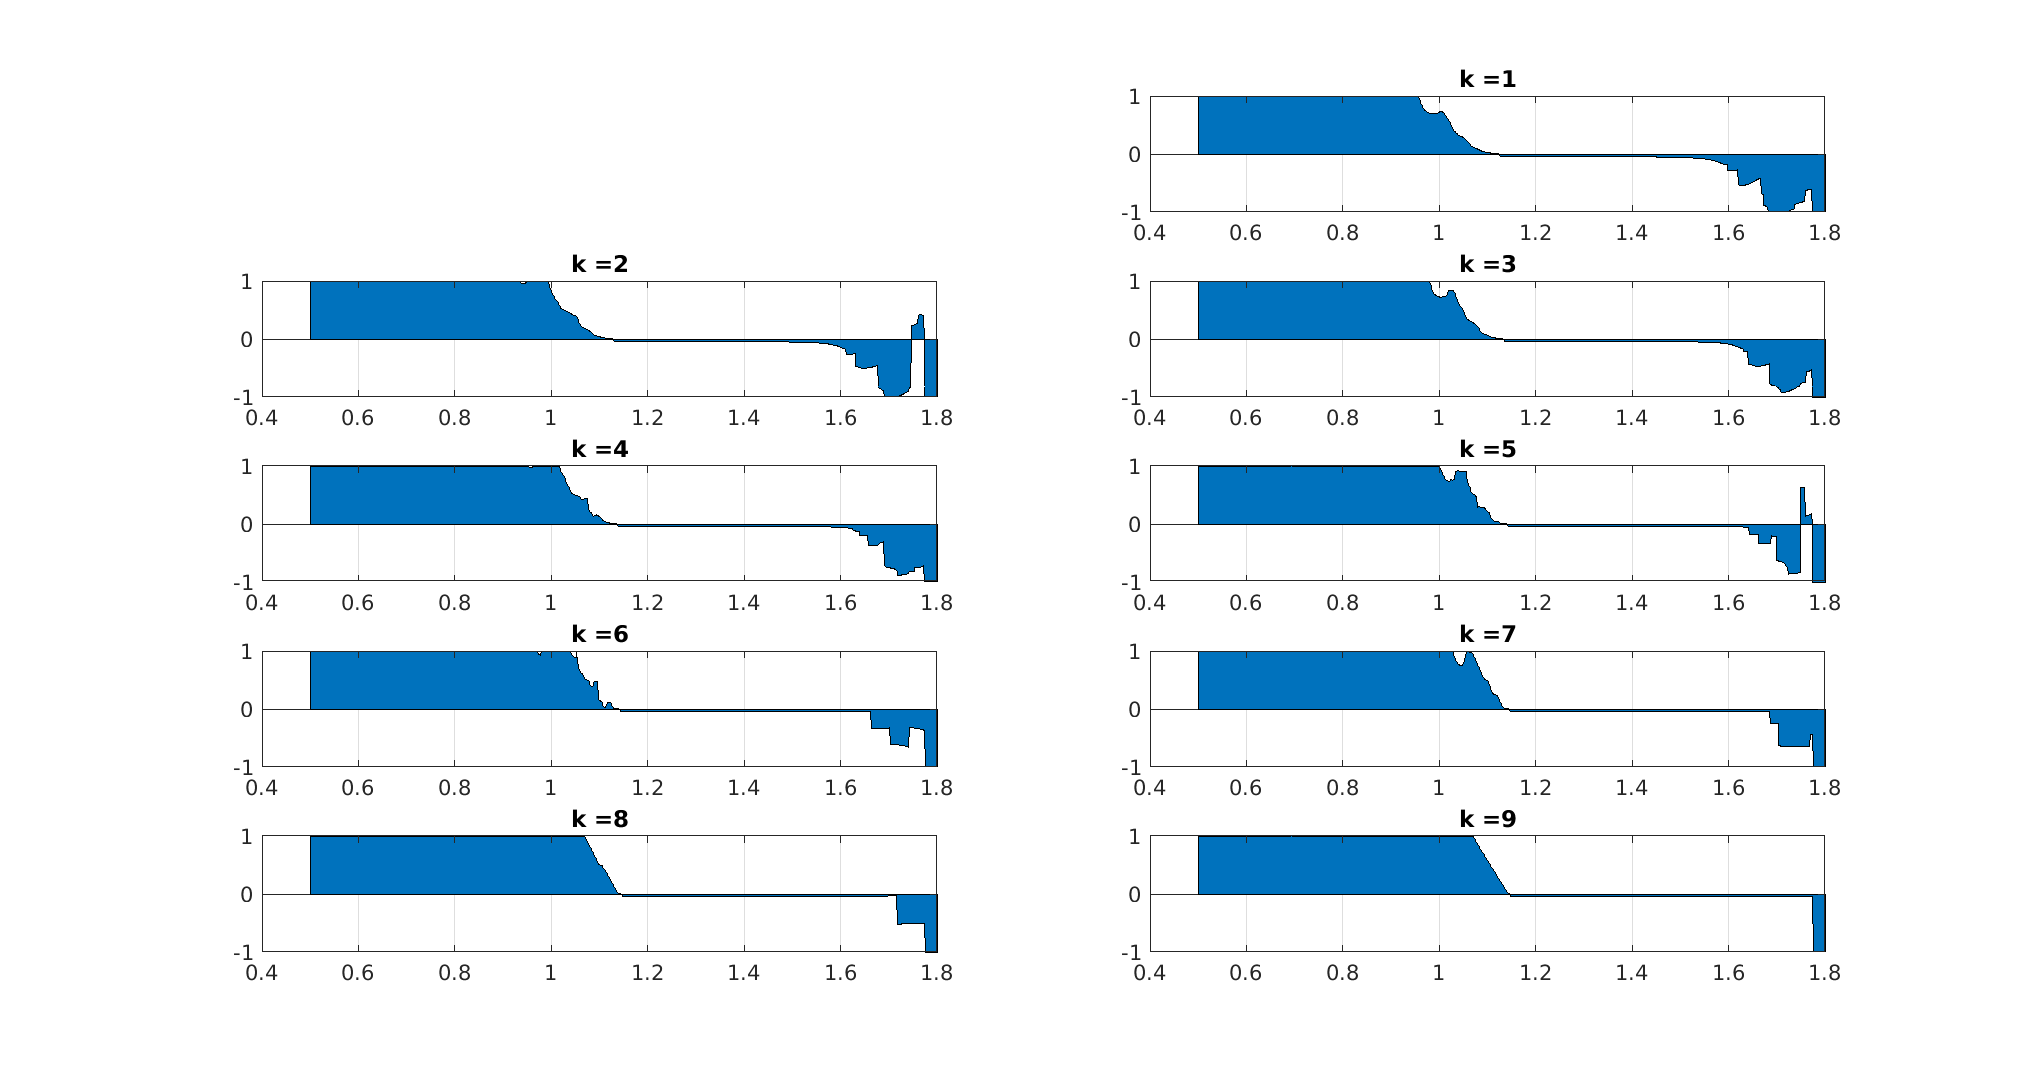
\includegraphics[scale = 0.5]{maps.png}

\begin{thebibliography}{9}
	
	\bibitem{PassTime}
	Peter Hieber, Matthias Scherer,
	\textit{A note on first-passage times of continuously time-changed Brownian motion},
	Statistics \& Probability Letters, Vol. 82 (2012), pp. 165–172,
	2012.
	
	\bibitem{Baldi}
	Paolo Baldi,
	\textit{Stochastic Calculus},
	Springer, 2017

\end{thebibliography}
\end{document}
